\documentclass[11pt]{article}

% 包导入
\usepackage[margin=1in]{geometry}
\usepackage{amsmath, amssymb}
\usepackage{graphicx}
\usepackage{hyperref}
\usepackage{float}
\usepackage{subcaption}
\usepackage{booktabs}

% 标题和作者信息
% 注意：如果是 Mini Course 学生，请使用下方注释的标题
\title{Homework 4: Convolutional Neural Networks}
% \title{Mini Course Homework 4} 
\author{
    [YIZHEN XU / yizhenxu] \\
}

\begin{document}

\maketitle

\section{Deliverable 1: Object Classification with CIFAR-100 Dataset}

\subsection{Custom Layer Test Cases}

The custom layers were validated against the official PyTorch implementations (\texttt{torch.nn.Conv2d} and \texttt{torch.nn.MaxPool2d}). To ensure an accurate comparison, weights and biases from the official layers were cloned directly to the custom layers. Forward pass outputs were then compared using \texttt{torch.allclose} with an absolute tolerance of $1\times 10^{-5}$.

\textbf{nn.Conv2d Test Cases:}
\begin{itemize}
    \item \textbf{Test Case 1 (Standard Convolution):} 
    Configuration: \texttt{kernel\_size=3, stride=1, padding=1, bias=True}. 
    Input shape: $(2, 3, 32, 32)$. The output successfully matched the official layer.
    
    \item \textbf{Test Case 2 (Downsampling Convolution):} 
    Configuration: \texttt{kernel\_size=5, stride=2, padding=0, bias=False}. 
    Input shape: $(4, 8, 28, 28)$. The output successfully matched the official layer.
\end{itemize}
\textbf{nn.MaxPool2d Test Cases:}
\begin{itemize}
    \item \textbf{Test Case 1 (Default Stride):} 
    Configuration: \texttt{kernel\_size=2, stride=None}. 
    Input shape: $(4, 16, 32, 32)$. The custom layer correctly defaulted the stride to 2, and the output shape $(4, 16, 16, 16)$ successfully matched the official layer exactly.
    
    \item \textbf{Test Case 2 (Overlapping Pooling):} 
    Configuration: \texttt{kernel\_size=3, stride=1}. 
    Input shape: $(2, 8, 14, 14)$. The custom layer successfully handled overlapping windows without padding, matching the official layer's output of $(2, 8, 12, 12)$.
\end{itemize}

\subsection{Fully Connected Neural Network (FCNN)}
\textbf{Max Accuracy:} 23.30\% \\
\textbf{Architecture \& Hyper-parameters:} 
\textbf{Architecture \& Hyper-parameters:} 
\begin{itemize}
    \item \textbf{Network Structure:} Flatten (3072) $\to$ Linear (1024) + ReLU $\to$ Linear (512) + ReLU $\to$ Linear (100).
    \item \textbf{Training Settings:} Adam optimizer ($\text{lr}=0.001$), Cross-Entropy Loss, Batch Size = 128, Epochs = 15.
\end{itemize}

\begin{figure}[H]
    \centering
    \begin{subfigure}{0.45\textwidth}
        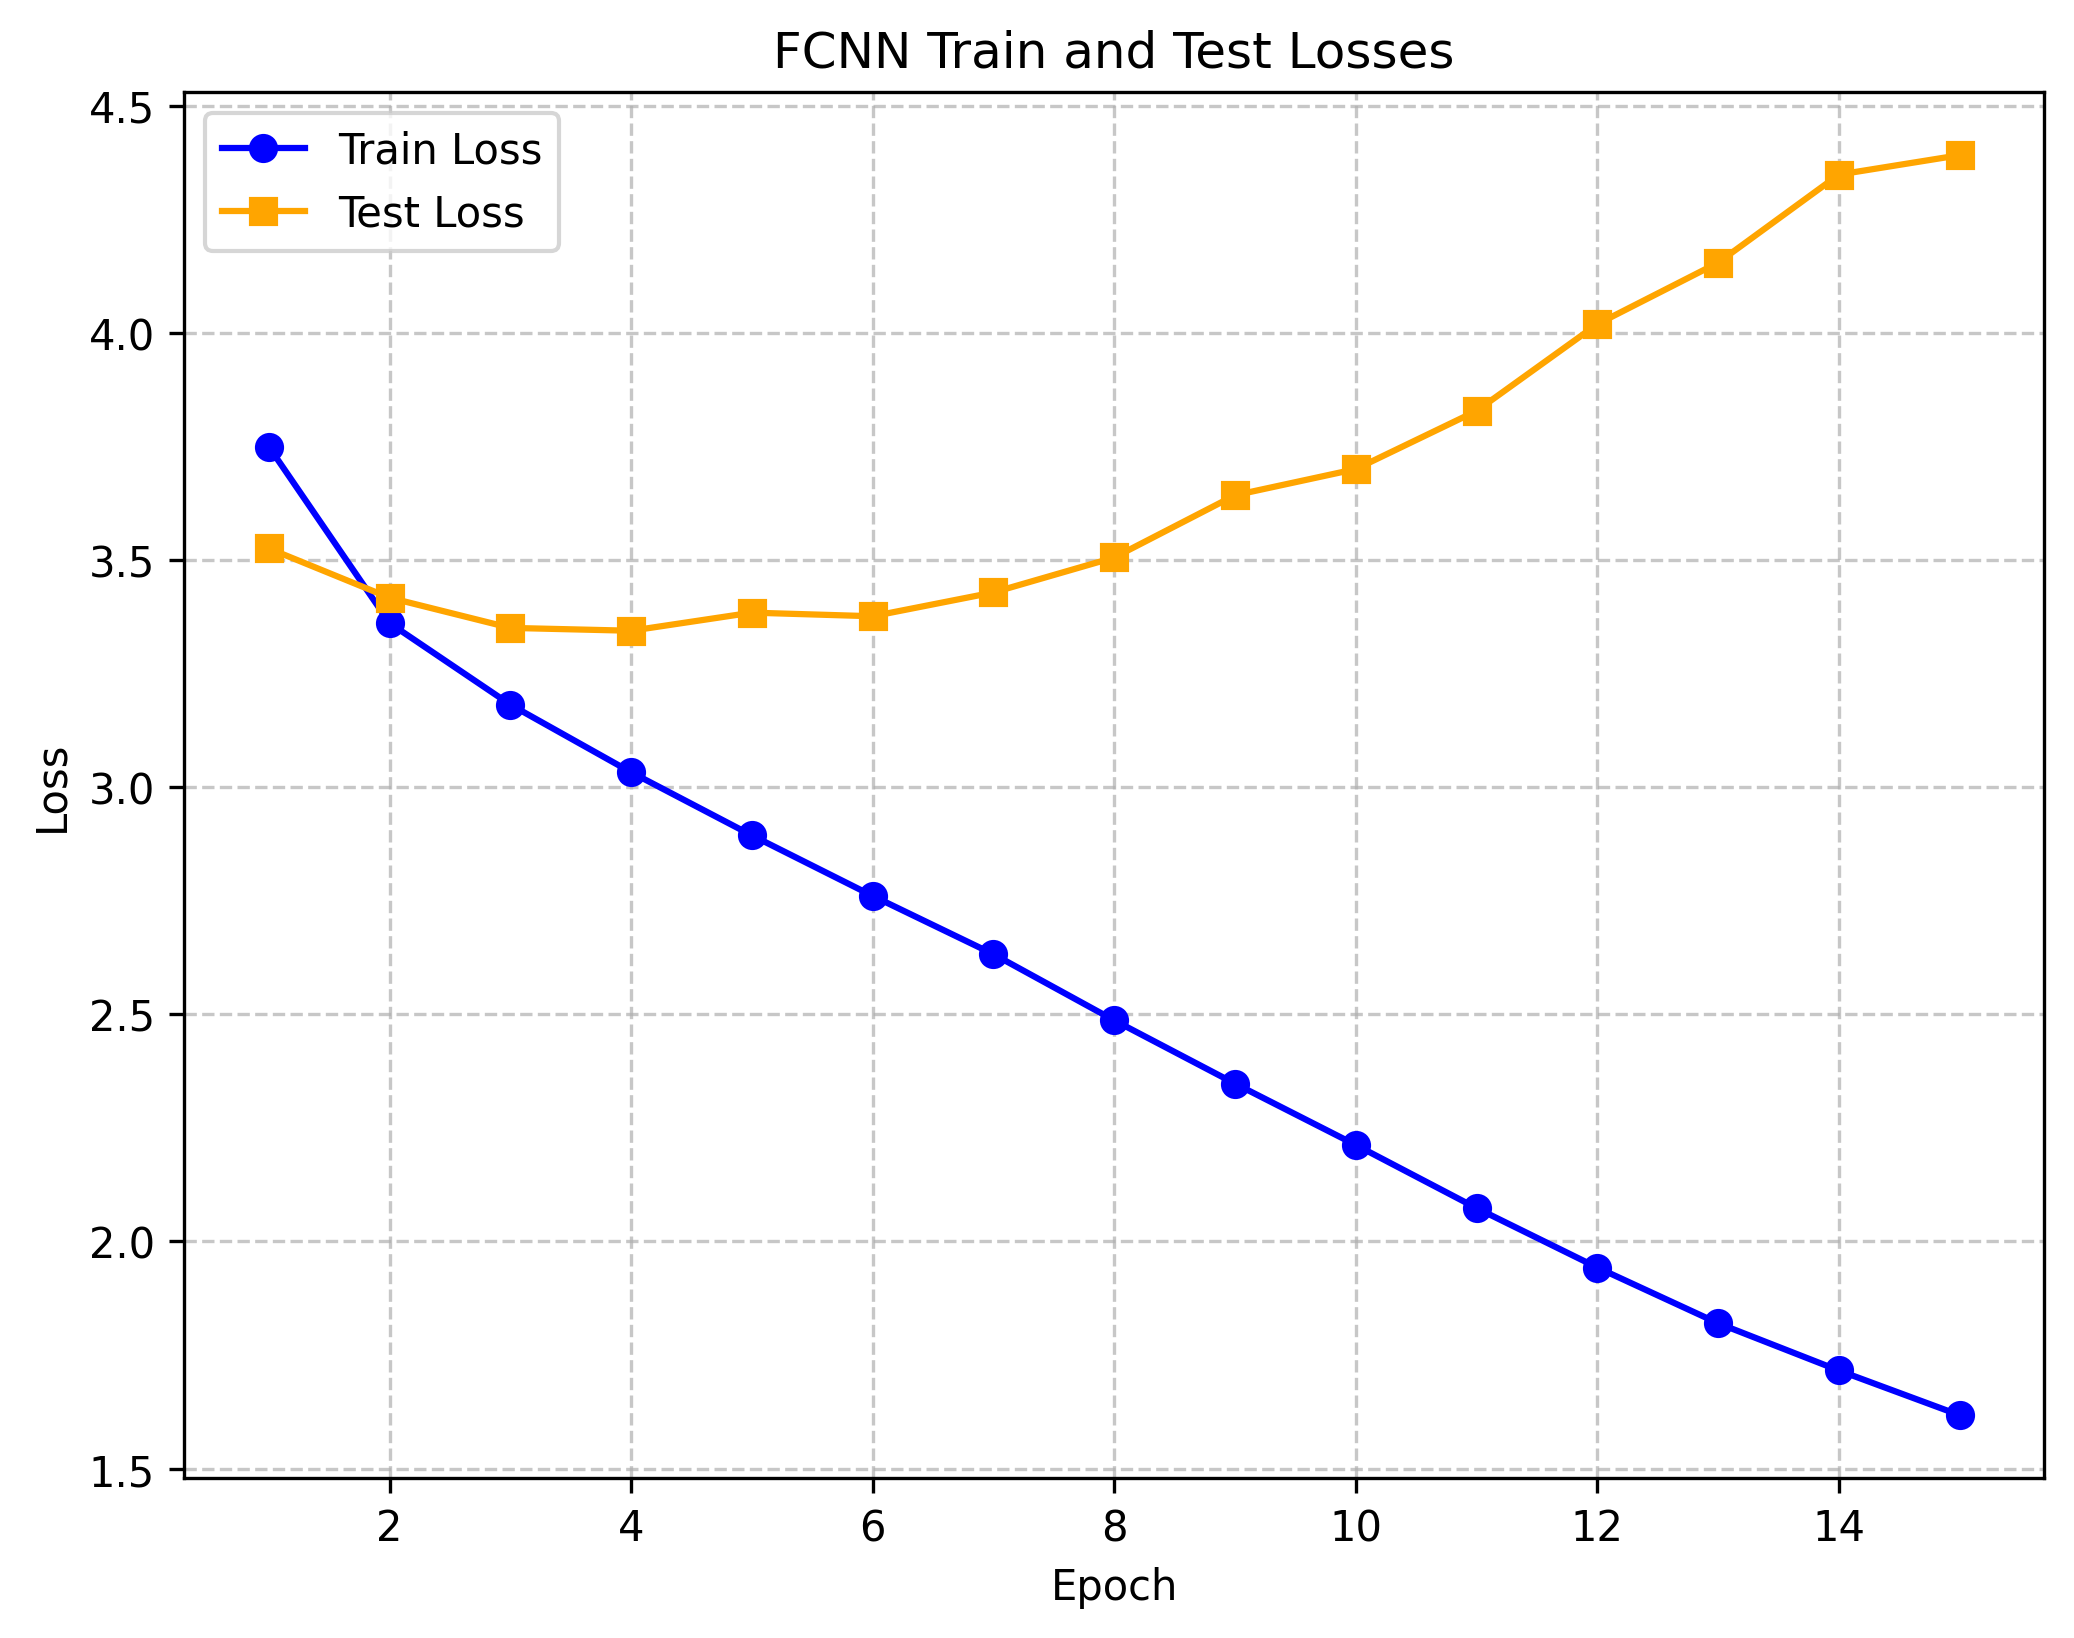
\includegraphics[width=\textwidth]{fcnn_loss_curve.png} 
        \caption{Train and Test Losses (FCNN)}
    \end{subfigure}
    \hfill
    \begin{subfigure}{0.45\textwidth}
        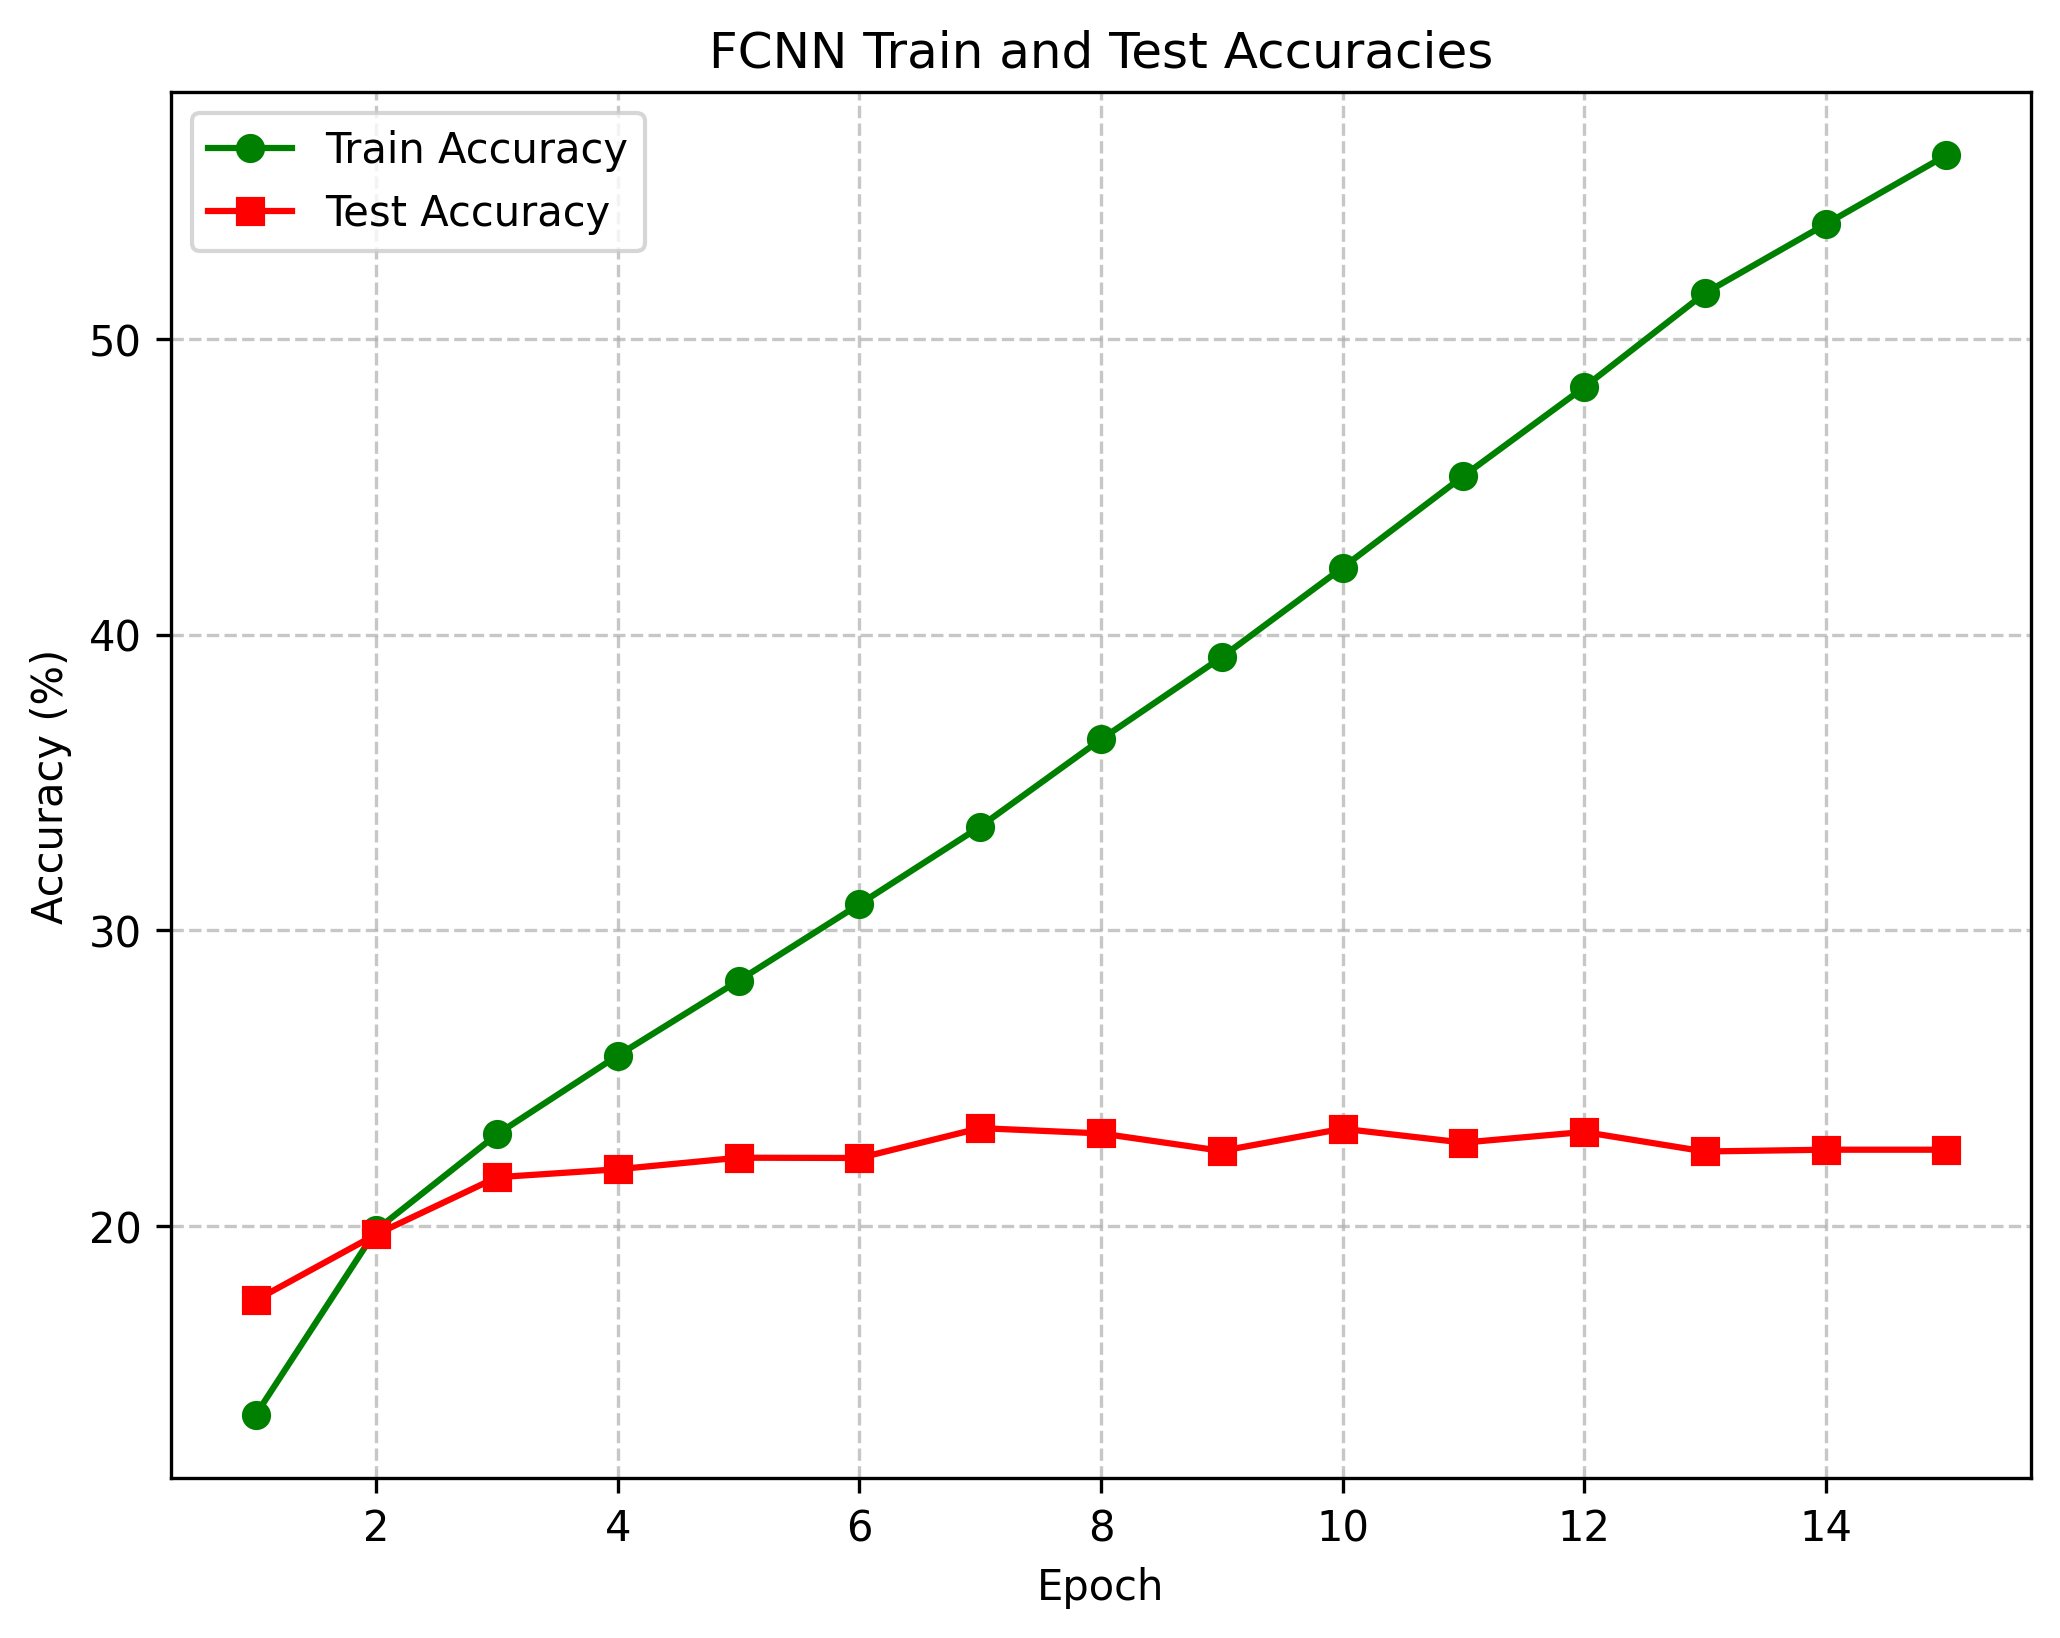
\includegraphics[width=\textwidth]{fcnn_acc_curve.png} 
        \caption{Train and Test Accuracies (FCNN)}
    \end{subfigure}
    \caption{Training Curves for Fully Connected Neural Network}
\end{figure}

\subsection{Convolutional Neural Network (CNN)}
\textbf{Max Accuracy:} 42.87\% \\
\textbf{Architecture \& Hyper-parameters:} 
\begin{itemize}
    \item \textbf{Feature Extractor:} \texttt{MyConv2D} (32 channels, $3\times3$, pad=1) + ReLU $\to$ \texttt{MyMaxPool2D} ($2\times2$, stride=2) $\to$ \texttt{MyConv2D} (64 channels, $3\times3$, pad=1) + ReLU $\to$ \texttt{MyMaxPool2D} ($2\times2$, stride=2).
    \item \textbf{Classifier:} Flatten ($64 \times 8 \times 8 \to 4096$) $\to$ Linear (512) + ReLU $\to$ Dropout ($p=0.5$) $\to$ Linear (100).
    \item \textbf{Training Settings:} Adam optimizer ($\text{lr}=0.001$), Cross-Entropy Loss, Batch Size = 128, Epochs = 15.
\end{itemize}

\begin{figure}[H]
    \centering
    \begin{subfigure}{0.45\textwidth}
        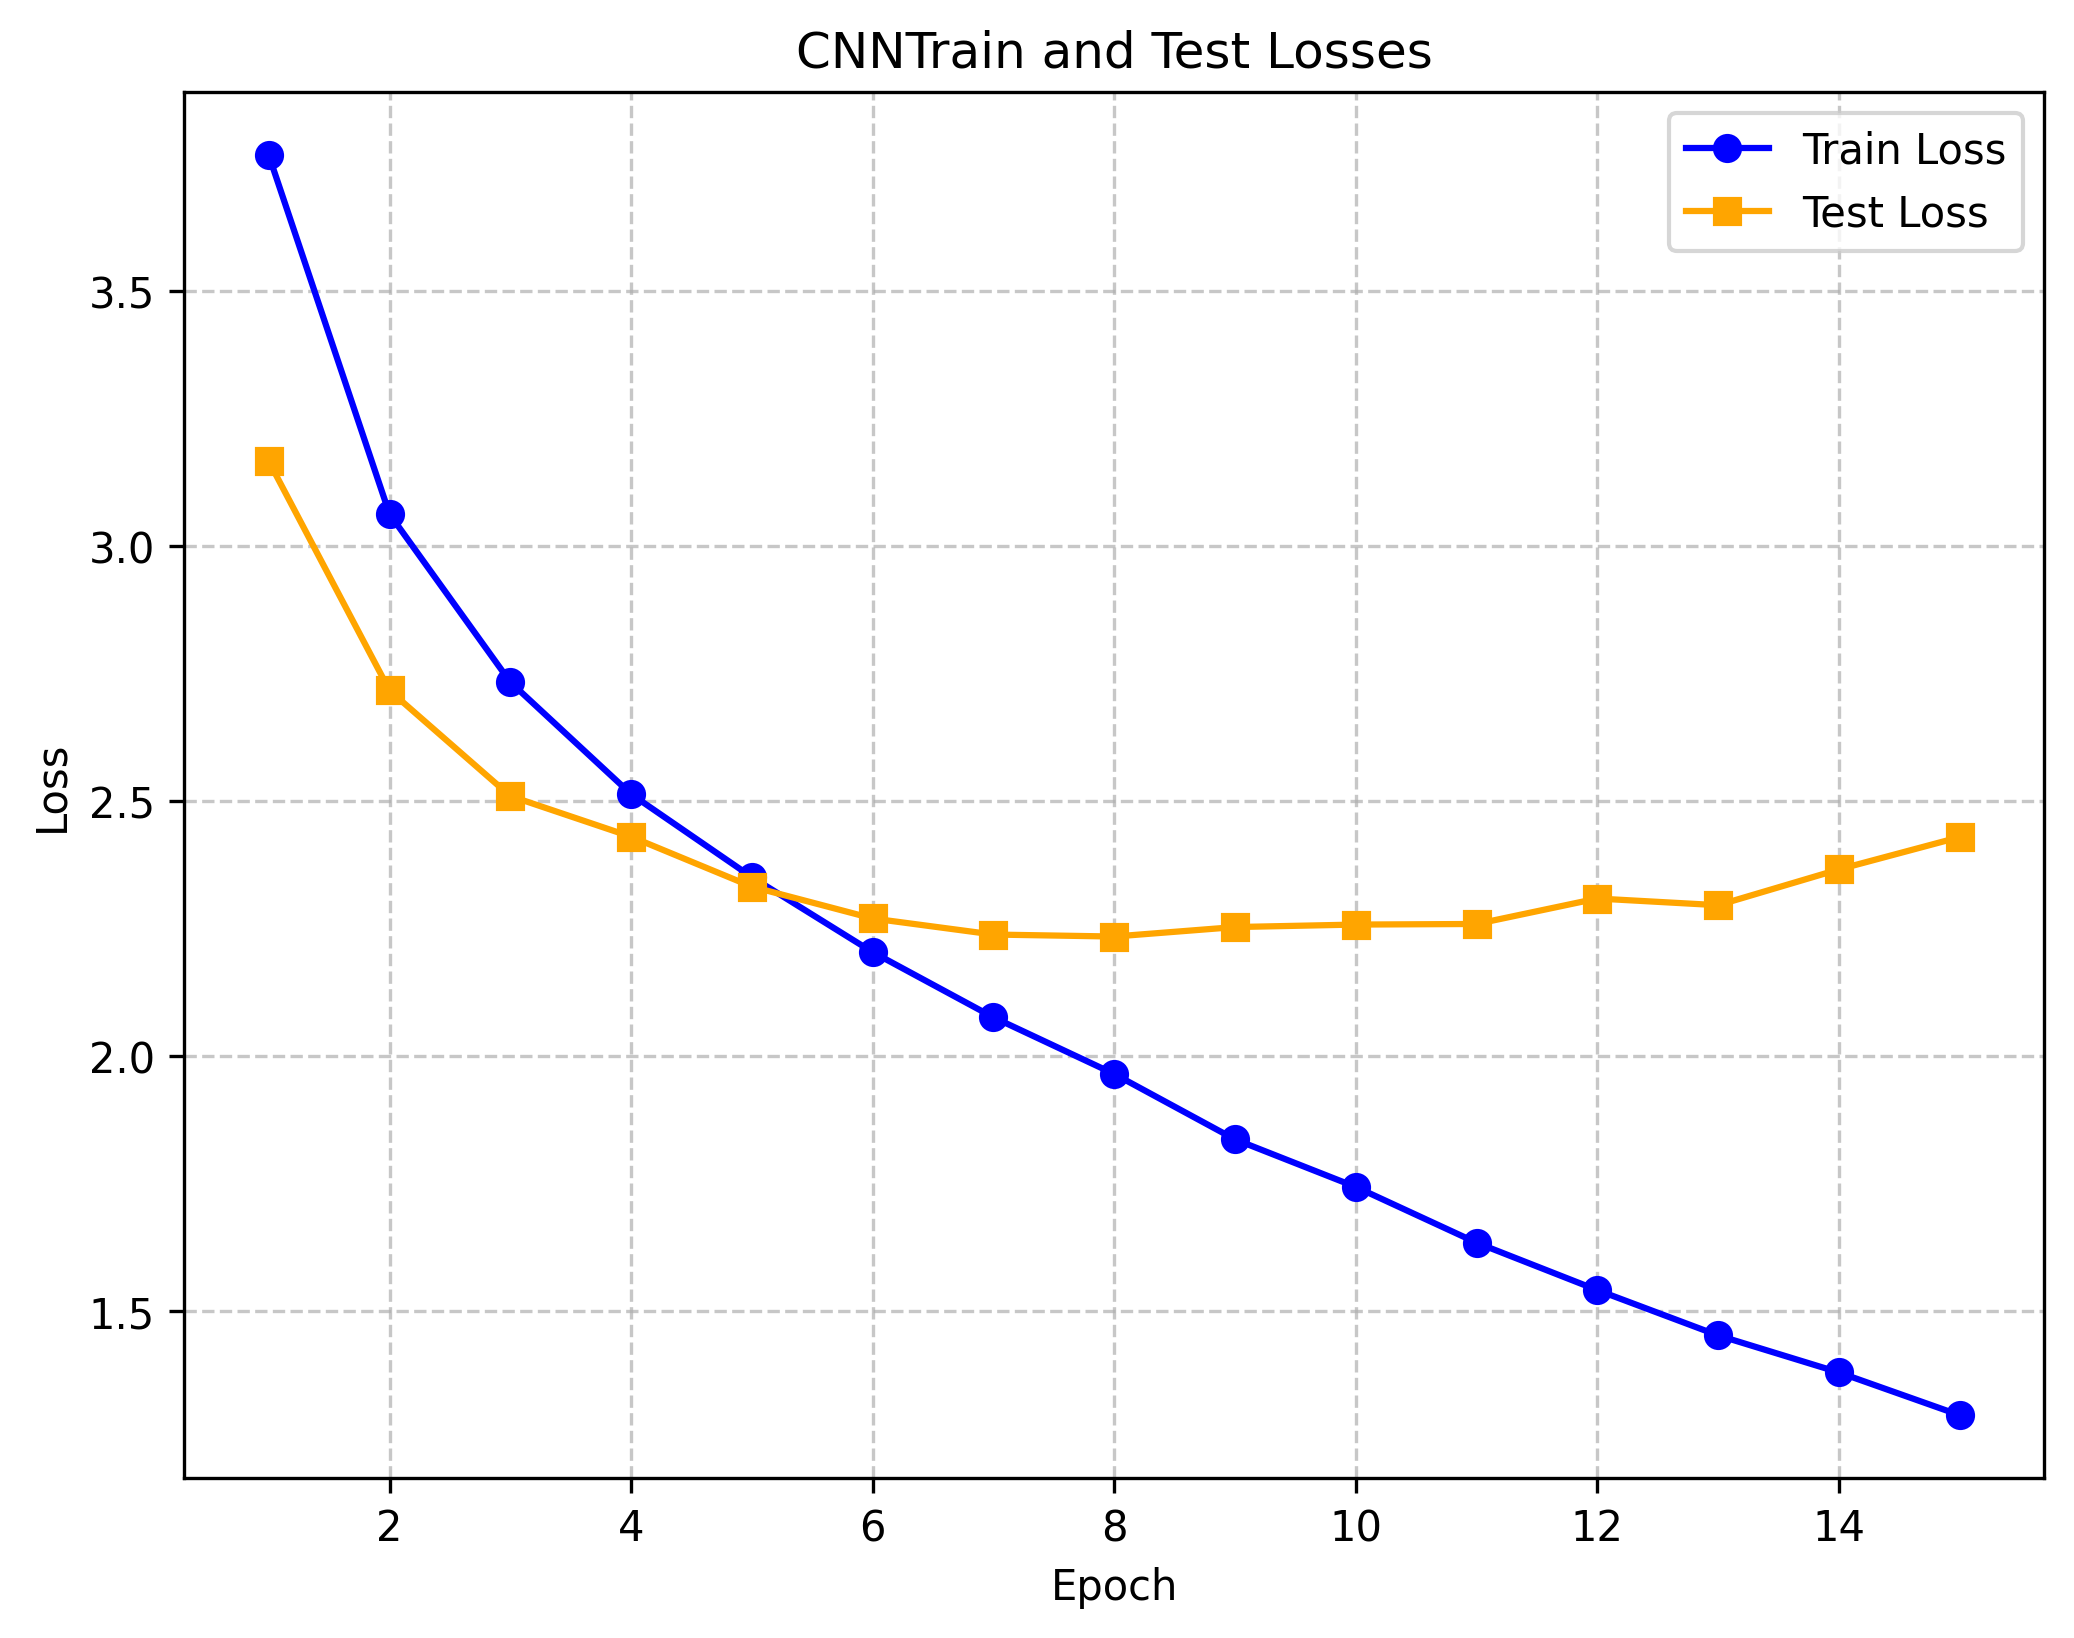
\includegraphics[width=\textwidth]{cnn_loss_curve.png} 
        \caption{Train and Test Losses (CNN)}
    \end{subfigure}
    \hfill
    \begin{subfigure}{0.45\textwidth}
        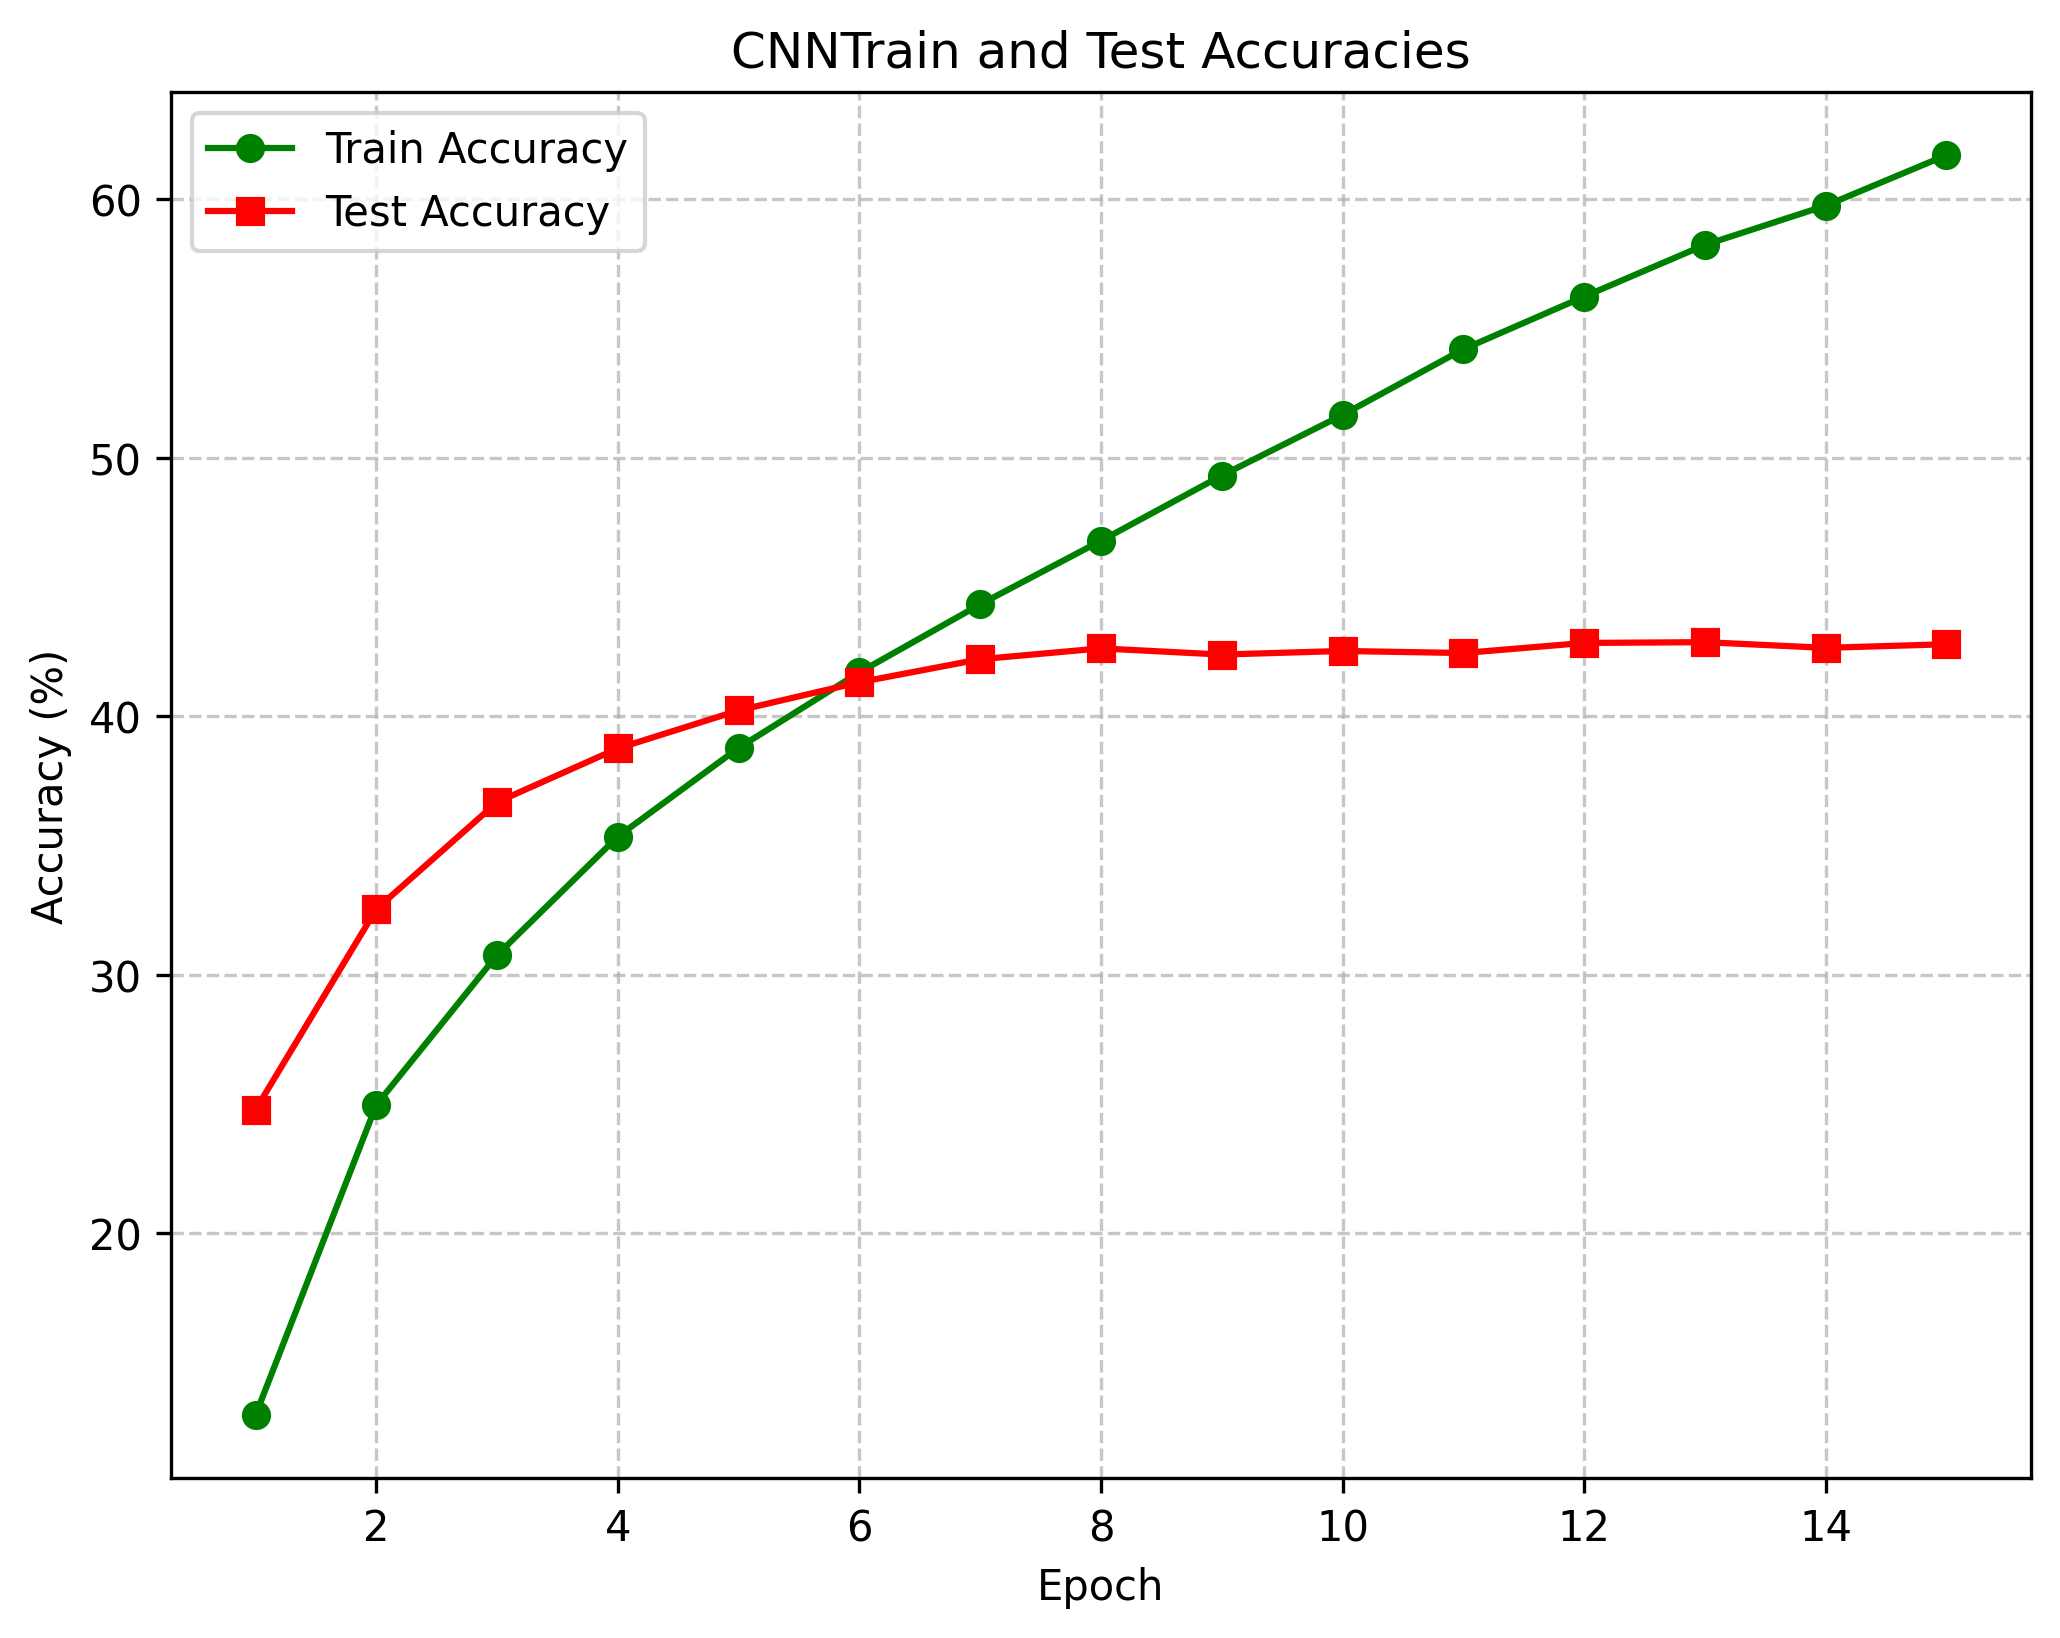
\includegraphics[width=\textwidth]{cnn_acc_curve.png} 
        \caption{Train and Test Accuracies (CNN)}
    \end{subfigure}
    \caption{Training Curves for Convolutional Neural Network}
\end{figure}

\subsection{Learning and Insights}
\begin{itemize}
    \item \textbf{Spatial Features:} The CNN significantly outperformed the FCNN. Convolutions preserve 2D spatial relationships (e.g., edges and textures), which are destroyed when images are prematurely flattened into 1D vectors.
    \item \textbf{Overfitting Mitigation:} Adding a Dropout layer ($p=0.5$) in the fully connected classifier effectively regularized the model and reduced the gap between training and validation accuracy.
    \item \textbf{Efficiency via \texttt{im2col}:} Custom convolutional layers are impractically slow with nested \texttt{for}-loops. Using \texttt{F.unfold} to convert sliding windows into matrix multiplications is essential for computational efficiency.
\end{itemize}

\subsection{Predictions Visualization}
% Visualization of FCNN and CNN predictions (5 random images with ground truth and predicted labels)

\begin{figure}[H]
    \centering
    % 插入5张FCNN的预测图
    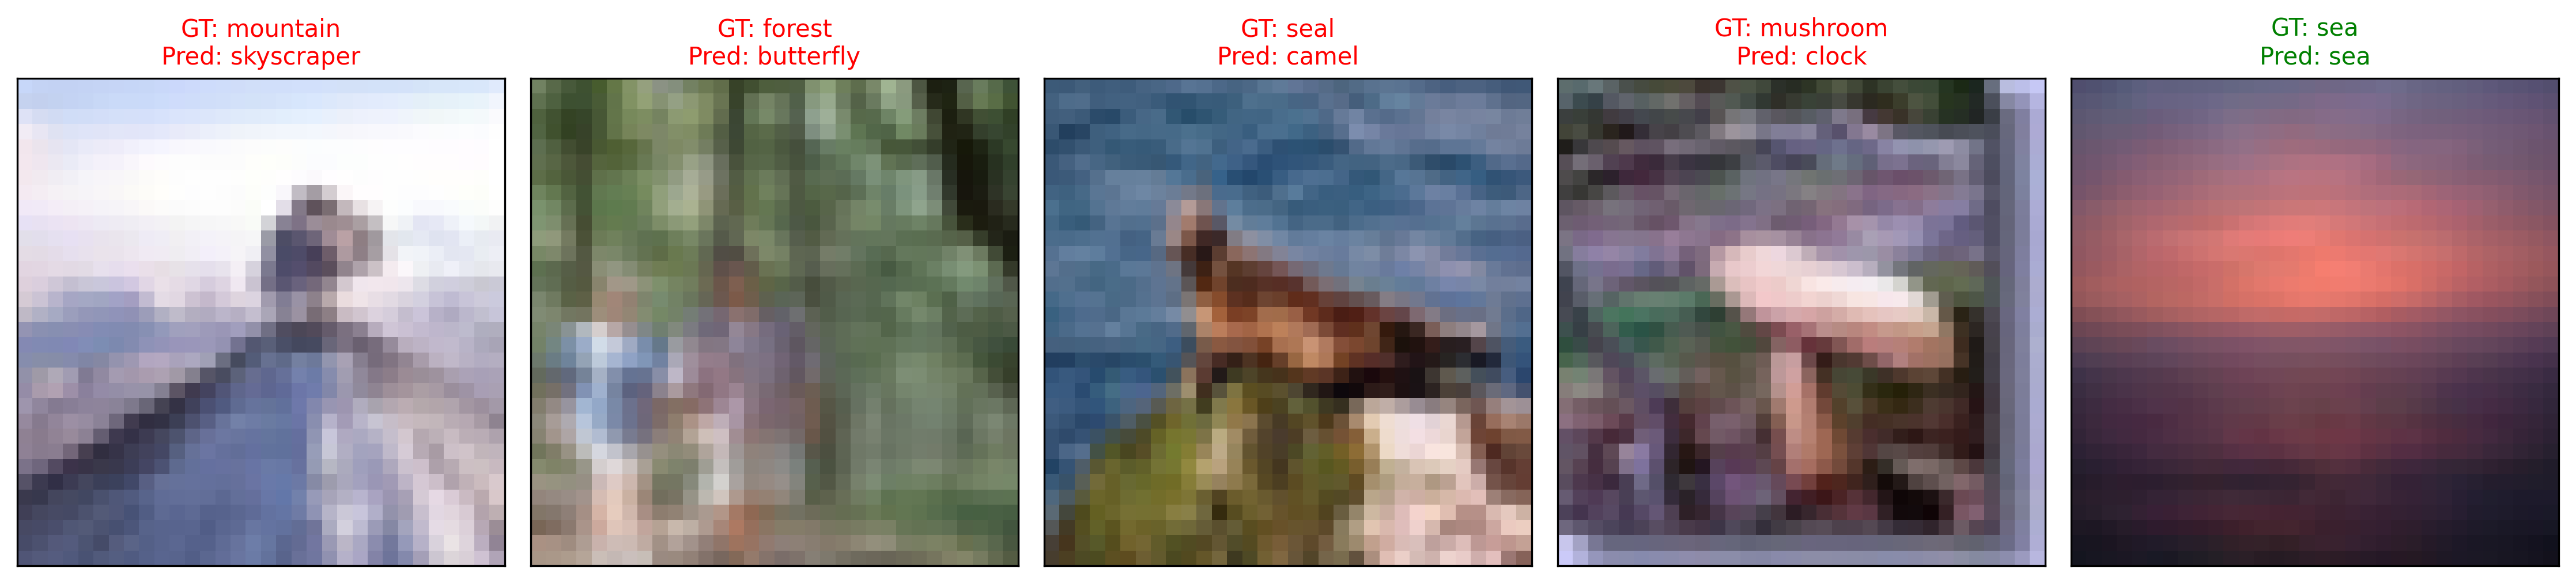
\includegraphics[width=0.8\textwidth]{fcnn_predictions.png} 
    \caption{FCNN Predictions.}
\end{figure}

\begin{figure}[H]
    \centering
    % 插入相同5张CNN的预测图
    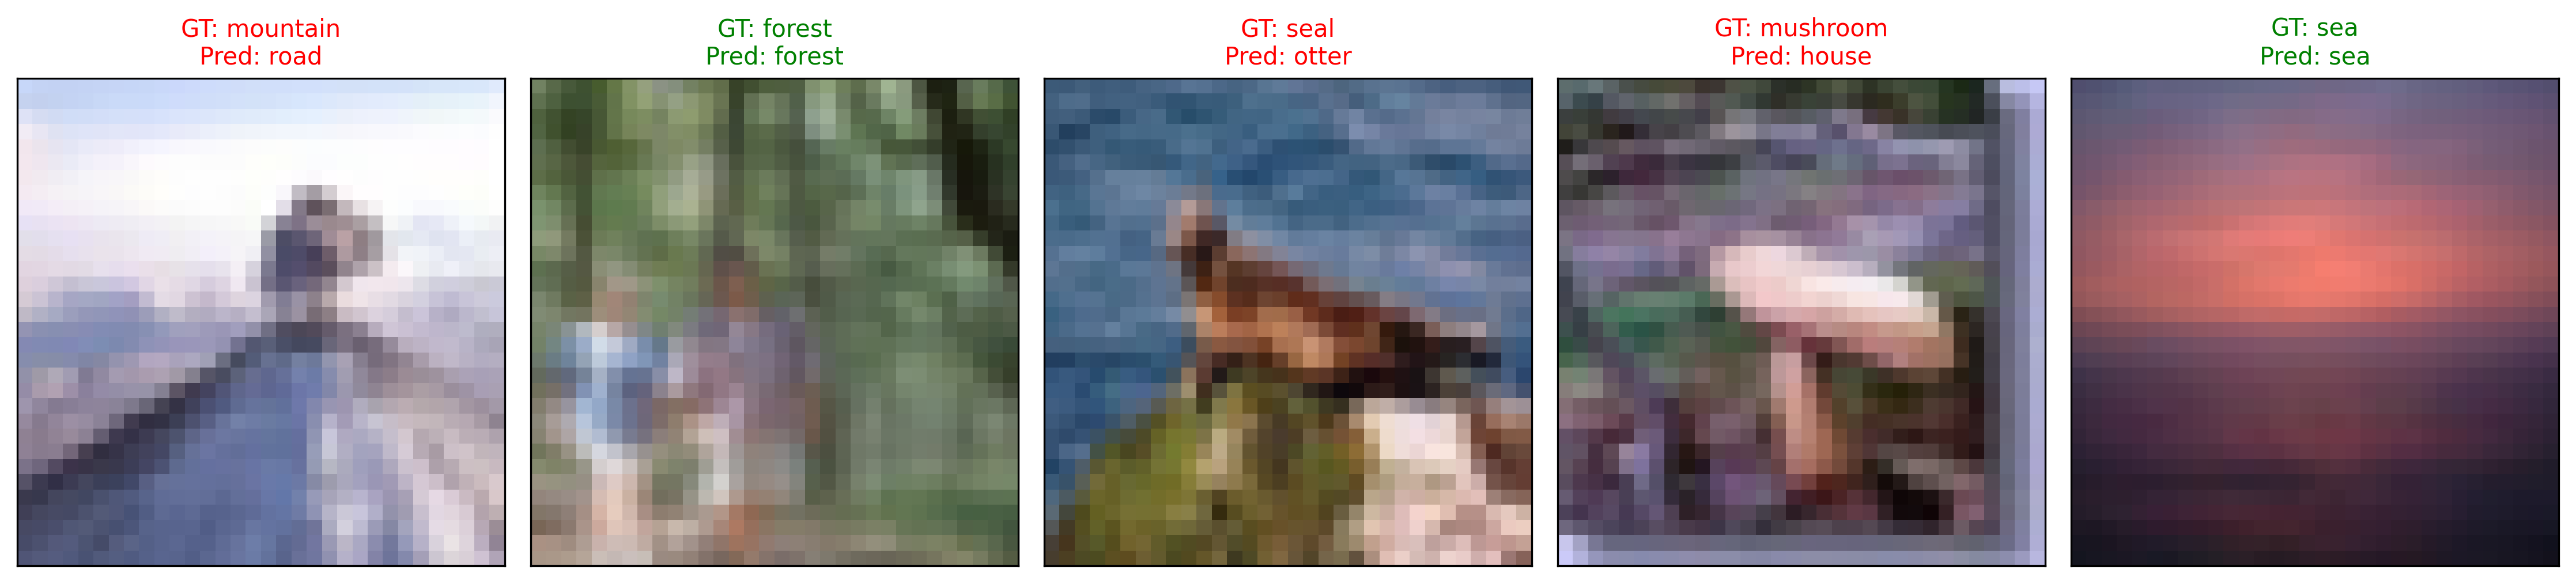
\includegraphics[width=0.8\textwidth]{cnn_predictions.png} 
    \caption{CNN Predictions.}
\end{figure}

\clearpage
% ---------------------------------------------------------
\section{Deliverable 2: Training for Optimal Results}

\subsection{Optimal Model Configurations}
\textbf{Max Accuracy:} 72.42\% \\
\textbf{Architecture \& Hyper-parameters:} 
\begin{itemize}
    \item \textbf{Feature Extractor:} \texttt{nn.Conv2d} (64 channels, $3\times3$, stride=1, pad=1) + \texttt{nn.BatchNorm2d} + ReLU $\to$ Stage 1 (2 $\times$ \texttt{BasicBlock}, 64, stride=1) $\to$ Stage 2 (2 $\times$ \texttt{BasicBlock}, 128, stride=2) $\to$ Stage 3 (2 $\times$ \texttt{BasicBlock}, 256, stride=2) $\to$ Stage 4 (2 $\times$ \texttt{BasicBlock}, 512, stride=2).
    \item \textbf{Classifier:} \texttt{nn.AdaptiveAvgPool2d} ($1 \times 1$) $\to$ Flatten ($512 \to 512$) $\to$ \texttt{nn.Linear} (100).
    \item \textbf{Training Settings:} Adam optimizer ($\text{lr}=0.001$, weight decay = $5 \times 10^{-4}$), \texttt{CosineAnnealingLR} scheduler, Batch Size = 128, Epochs = 60.
    \item \textbf{Regularization:} \texttt{RandomCrop} (size=32, padding=4), \texttt{RandomHorizontalFlip}, \texttt{RandomRotation}.
\end{itemize}

\begin{figure}[H]
    \centering
    \begin{subfigure}{0.45\textwidth}
        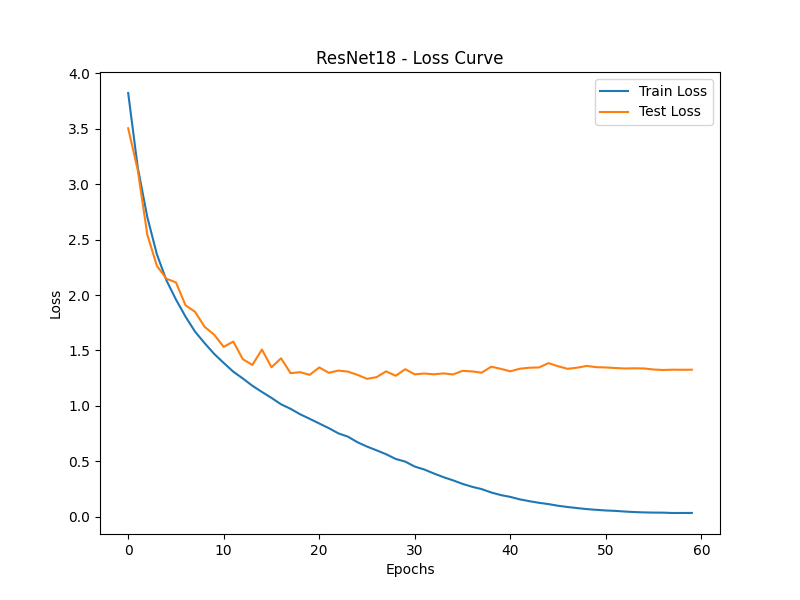
\includegraphics[width=\textwidth]{resnet_loss_curve.png} % 替换为 Loss 图
        \caption{Train and Test Losses}
    \end{subfigure}
    \hfill
    \begin{subfigure}{0.45\textwidth}
        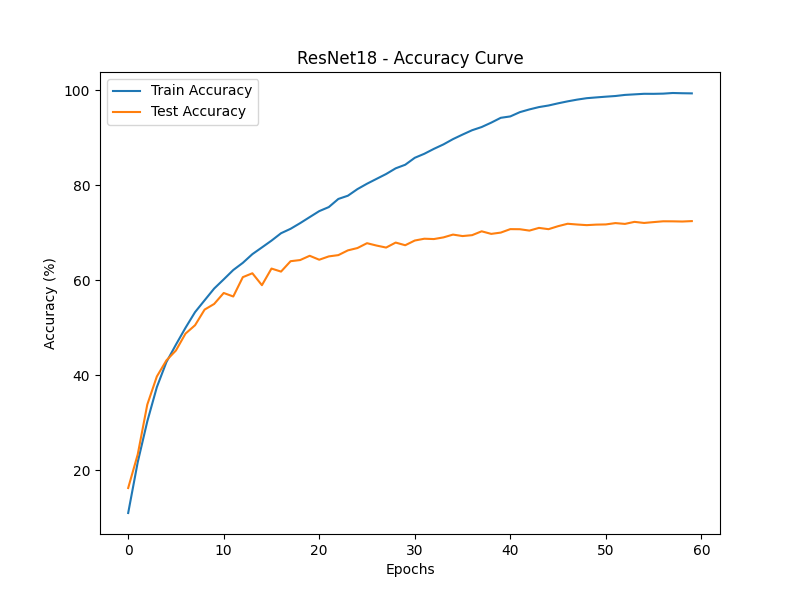
\includegraphics[width=\textwidth]{resnet_acc_curve.png} % 替换为 Accuracy 图
        \caption{Train and Test Accuracies}
    \end{subfigure}
    \caption{Training Curves for Optimal Model}
\end{figure}

\subsection{Visualizations of Results}
% Visualization of results and number of correct predictions visually out of 10
\begin{figure}[H]
    \centering
    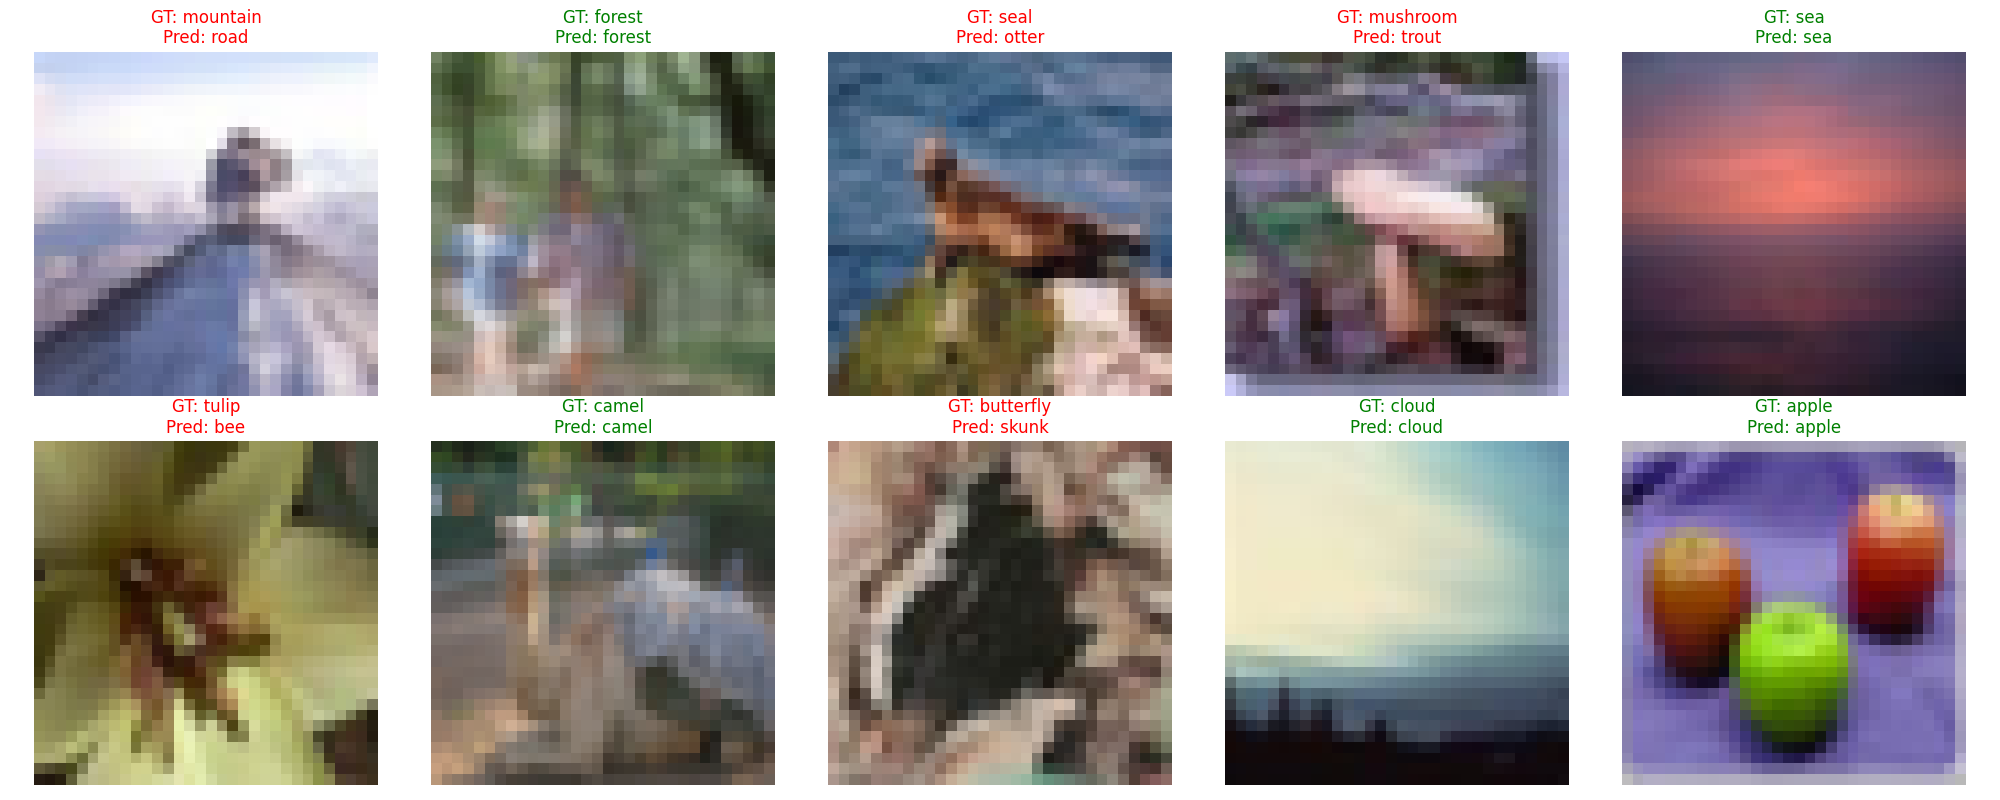
\includegraphics[width=0.8\textwidth]{resnet_predictions.png} % 替换为 10 张图的预测结果
    \caption{Optimal Model Predictions on 10 Random Images.}
\end{figure}

\subsection{Learning and Insights}
\begin{itemize}
    \item \textbf{Regularization via Data Augmentation:} The addition of spatial data augmentations (Random Crop, Horizontal Flip, Random Rotation) significantly increased the difficulty of the training data. This effectively eliminated overfitting, evidenced by the inverted accuracy gap where the model performed better on the clean, unaugmented test set ($47.21\%$) than on the distorted training set ($39.44\%$).
    \item \textbf{Capacity Bottleneck (Underfitting):} Despite the stabilization provided by the Cosine Annealing scheduler and the regularization from data augmentation, the simple CNN's performance plateaued at $\sim 47\%$. This indicated a severe underfitting scenario: the shallow architecture lacked the requisite parameter capacity and receptive field depth to extract sufficiently complex features for a 100-class classification task.
    \item \textbf{Necessity of Residual Connections:} Upgrading to the ResNet-18 architecture resolved the capacity bottleneck. The residual connections ($F(x) + x$) allowed for training a significantly deeper network without gradient degradation, capturing multi-scale spatial features and boosting the test accuracy to above 60\%.
\end{itemize}

\subsection{Ablation Study}
% Write a brief and informal ablation study report
\begin{table}[H]
    \centering
    \begin{tabular}{llc}
        \toprule
        \textbf{Model / Configuration} & \textbf{Change Description} & \textbf{Validation Accuracy} \\
        \midrule
        Baseline CNN & Initial setup from Del 1 & 42.87\% \\
        + Data Aug. \& LR Scheduler & Added RandomCrop, Flip, & 47.21\% \\
        & Rotation and CosineAnnealingLR & \\
        + ResNet18 Architecture & Changed to deeper residual network & 72.42\% \\
        \bottomrule
    \end{tabular}
    \caption{Ablation Study of Model Architectures and Training Techniques on CIFAR-100.}
    \label{tab:ablation}
\end{table}

\clearpage
% ---------------------------------------------------------
\section{Deliverable 3: Naive Object Detection}

\subsection{Methodology and Implementation}
Object detection was approached by extending a pre-trained image classifier into a localization framework. The primary objective was to identify and bound target objects (cats and dogs) within high-resolution images.

\subsubsection{Baseline: Fixed Grid Partitioning}
A baseline was established by partitioning the input image into a rigid $5 \times 5$ grid of non-overlapping patches. Each patch was processed through a ResNet-50 classifier pre-trained on the ImageNet-1K dataset. A detection was recorded if the classifier's confidence score for a relevant object class exceeded a predefined threshold. However, this method was found to be highly susceptible to alignment errors; target objects bisected by grid boundaries often failed to trigger a detection, as only partial features were presented to the classifier.

\subsubsection{Improved Method: Sliding Window and NMS}
To overcome the limitations of the baseline, a more robust detection pipeline was developed:
\begin{itemize}
    \item \textbf{Sliding Window Mechanism:} A sliding window approach was utilized with a defined stride to ensure comprehensive and overlapping coverage of the image. Multiple window scales were employed to accommodate the varying sizes of animals present in the frames.
    \item \textbf{Categorical Mapping:} Given the fine-grained nature of ImageNet labels, a keyword-based mapping system was integrated. Specific breeds (e.g., \textit{terrier, tabby}) were automatically aggregated into broader "Dog" or "Cat" categories based on their class indices.
    \item \textbf{Non-Maximum Suppression (NMS):} To resolve the issue of redundant bounding boxes generated by the overlapping windows, a Non-Maximum Suppression (NMS) algorithm was implemented. The Intersection over Union (IoU) between candidate boxes was calculated, and boxes with lower confidence scores were suppressed. This ensured that only the most precise bounding box was retained for each detected entity.
\end{itemize}

\subsection{Detection Results}
% The two images annotated with bounding boxes
\begin{figure}[H]
    \centering
    \begin{subfigure}{0.45\textwidth}
        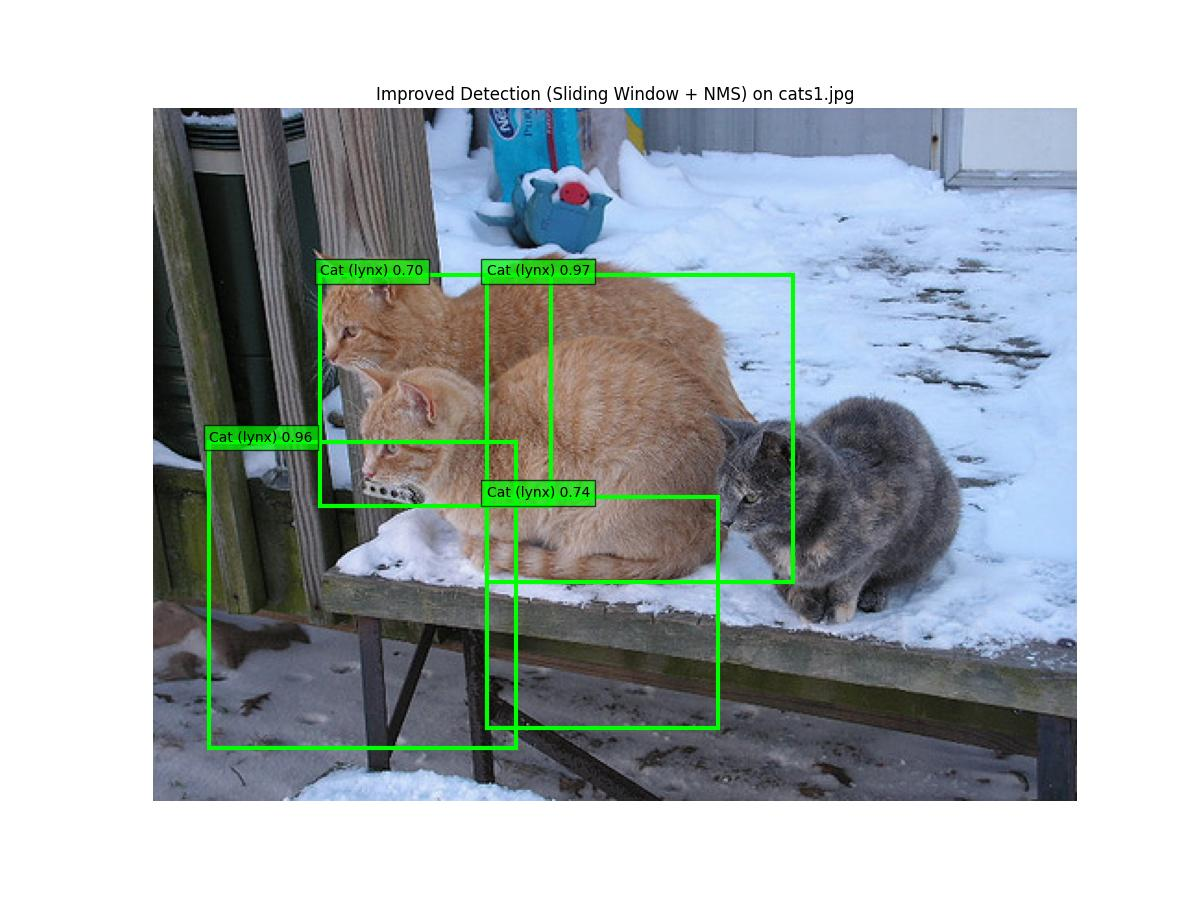
\includegraphics[width=\textwidth]{improved_cats1.jpg} % 替换为带 bounding box 的猫图
        \caption{Detection result for Cat image}
    \end{subfigure}
    \hfill
    \begin{subfigure}{0.45\textwidth}
        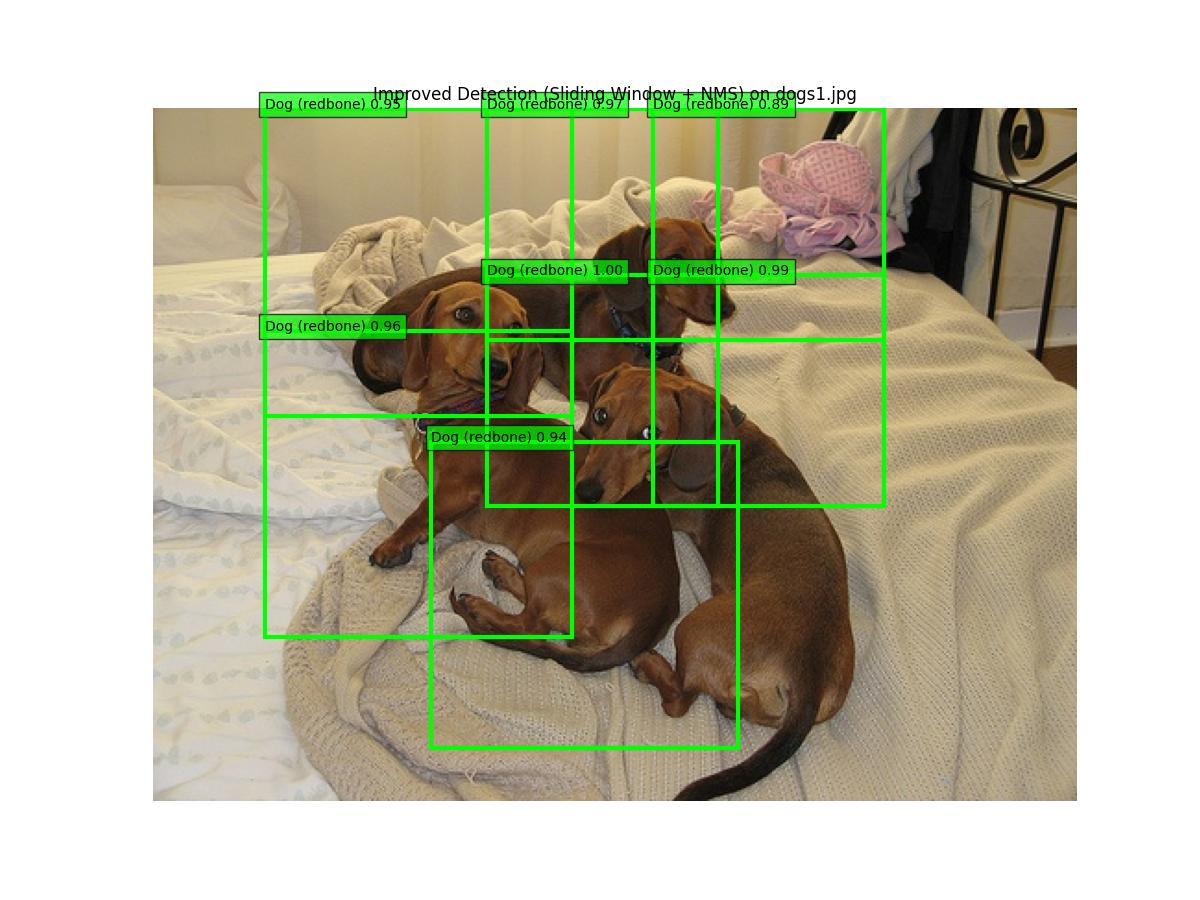
\includegraphics[width=\textwidth]{improved_dogs1 (1).jpg} % 替换为带 bounding box 的狗图
        \caption{Detection result for Dog image}
    \end{subfigure}
    \caption{Naive Object Detection using Classifier Patches}
\end{figure}

\clearpage
% ---------------------------------------------------------
\section{Deliverable 4: Performance Profiling}

% Measure mAP50 and latency

\subsection{Experimental Setup and Metrics}
The performance of YOLOv8n and Faster R-CNN was evaluated using a randomly sampled subset of 100 images from the COCO 2017 validation dataset. Two primary metrics were recorded: mean Average Precision at an IoU threshold of 0.5 ($mAP_{50}$) and inference latency. The latency was measured as the average time required to process a single image with a batch size of 1.

\subsection{Results and Analysis}
The empirical results are summarized in Table \ref{table:performance}.

\begin{table}[H]
\centering
\caption{Performance and Latency Comparison on COCO 2017 Val (100 Samples)}
\label{table:performance}
\begin{tabular}{lcc}
\toprule
\textbf{Model Architecture} & \textbf{$mAP_{50}$} & \textbf{Avg Latency (s)} \\ 
\midrule
YOLOv8n (Single-stage)      & 0.5839              & 0.0076                   \\
Faster R-CNN (Two-stage)    & 0.6931              & 0.0791                   \\ 
\bottomrule
\end{tabular}
\end{table}

A significant trade-off between localization precision and computational efficiency was observed:
\begin{itemize}
    \item \textbf{Inference Efficiency:} YOLOv8n exhibited a high degree of efficiency, achieving a latency of approximately 7.6 ms per image. This rapid inference is attributed to its single-stage architecture, which predicts bounding boxes and class probabilities in a single forward pass.
    \item \textbf{Detection Precision:} Faster R-CNN achieved a superior $mAP_{50}$ of 0.6931, representing an approximately 18.7\% improvement over YOLOv8n. This enhancement is facilitated by the Region Proposal Network (RPN) and the subsequent refinement stages, which allow for more precise feature extraction and object localization.
\end{itemize}

\subsection{Conclusion}
The results confirm that while YOLOv8n is highly suitable for real-time applications requiring minimal latency, Faster R-CNN remains more effective for tasks where detection accuracy is prioritized over processing speed. The observed 10-fold difference in latency underscores the architectural distinctions between single-stage and two-stage detection frameworks.

\clearpage
% ---------------------------------------------------------
\section{Deliverable 5: Modern Open Vocabulary Object Detection}

\subsection{YOLOv8s-world Evaluation on COCO}
The YOLOv8s-world model was evaluated on 100 random COCO 2017 validation images. The vocabulary was dynamically set to the 80 COCO classes using \texttt{model.set\_classes()}. A manual mAP50 of \textbf{0.5558} was obtained, demonstrating the model's zero-shot capability to align visual features with text prompts without fixed-label training.

\subsection{Prompt-based Detection and Visualization}
Specific prompts ("cat", "dog") were utilized for inference on target images. As shown in Figure \ref{fig:yolo_world}, all three cats and three dogs were successfully localized. The results confirm that YOLOv8s-world effectively translates semantic descriptions into precise bounding boxes.

\begin{figure}[H]
    \centering
    \begin{subfigure}[b]{0.45\textwidth}
        \centering
        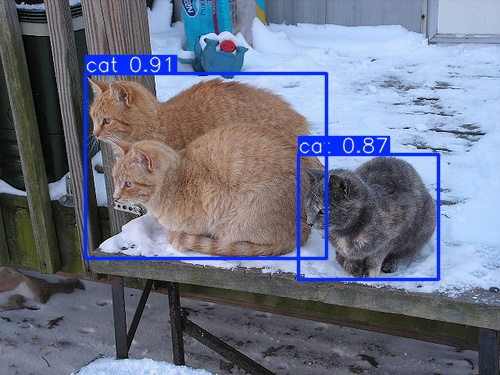
\includegraphics[width=\textwidth]{cats1.jpg}
        \caption{YOLOv8s-world on \texttt{cats1.jpg}}
    \end{subfigure}
    \hfill
    \begin{subfigure}[b]{0.45\textwidth}
        \centering
        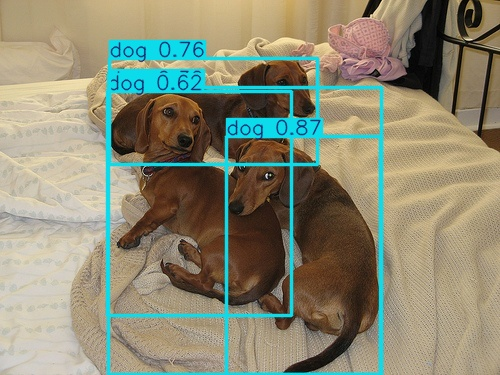
\includegraphics[width=\textwidth]{dogs1.jpg}
        \caption{YOLOv8s-world on \texttt{dogs1.jpg}}
    \end{subfigure}
    \caption{Open-Vocabulary detection results generated by YOLOv8s-world.}
    \label{fig:yolo_world}
\end{figure}

\subsection{LVLM Detection and Architectural Comparison}
The same images were processed by the Gemini 3 Flash model (LVLM). As shown in Figure \ref{fig:lvlm_viz}, the LVLM also generated high-quality visualizations with annotated bounding boxes, correctly identifying all six instances across both scenarios. 

\begin{figure}[H]
    \centering
    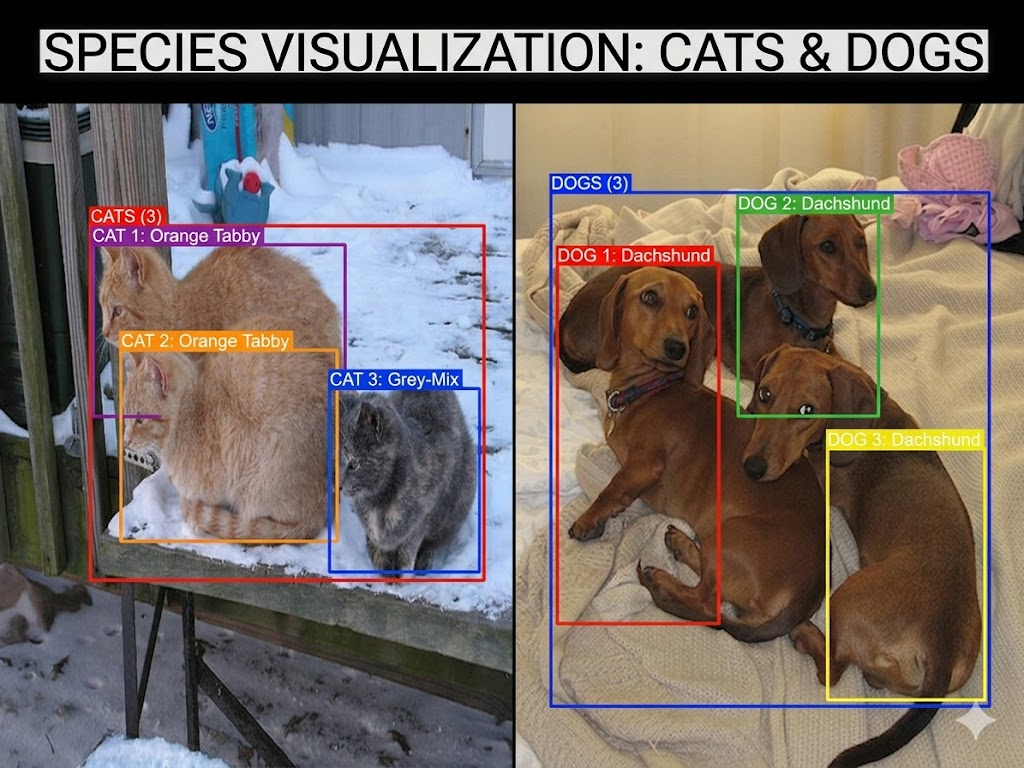
\includegraphics[width=\textwidth]{gemini_detection.jpg}
    \caption{Detection results generated and visualized by the Gemini 3 Flash model.}
    \label{fig:lvlm_viz}
\end{figure}

\subsection{LVLM Comparison and Architectural Analysis}
The same images were processed by the Gemini 3 Flash model (LVLM). Both models identified the correct number of instances, but distinct architectural methodologies were observed:
\begin{itemize}
    \item \textbf{YOLOv8s-world:} Utilizes a shared latent space for vision-language alignment, offering high efficiency and real-time inference capability.
    \item \textbf{LVLM:} Leverages a large-scale transformer to regress coordinates as part of a generative sequence, providing superior semantic robustness in complex scenarios.
\end{itemize}

\appendix
\section{LVLM Raw Response (Task 5.3)}
\begin{itemize}
 This visualization accurately identifies the animals in both images. The left panel shows the three cats, each with an individual box indicating its color/pattern, and a larger box for the total cat count. The right panel displays the three dogs, all labeled as dachshunds, with a matching box for the total count.
\end{itemize}

\end{document}